\documentclass[11pt, oneside]{article}   	% use "amsart" instead of "article" for AMSLaTeX format
\usepackage{geometry}                		% See geometry.pdf to learn the layout options. There are lots.
\geometry{a4paper}                   		% ... or a4paper or a5paper or ... 
\pagestyle{empty}

\usepackage{graphicx}				% Use pdf, png, jpg, or eps§ with pdflatex; use eps in DVI mode							
\usepackage{amssymb}
\usepackage{tikz}
\usetikzlibrary{shapes.geometric, arrows}

\tikzstyle{startstop} = [trapezium, 
trapezium stretches=true, % A later addition
trapezium left angle=70, 
trapezium right angle=110, 
minimum width=3cm, 
minimum height=1cm, text centered, 
draw=black, fill=blue!30]


\tikzstyle{io} = [rectangle, rounded corners, 
minimum width=3cm, 
minimum height=1cm,
text centered,
text width=6cm, 
draw=black, 
fill=red!30]

\tikzstyle{create} = [rectangle, rounded corners, 
minimum width=3cm, 
minimum height=1cm, 
text centered, 
text width=5cm, 
draw=black, 
fill=orange!30]

\tikzstyle{run} = [rectangle, rounded corners, 
minimum width=3cm, 
minimum height=1cm, 
text centered, 
text width=7cm, 
draw=black, 
fill=green!30]

\tikzstyle{decision} = [diamond, 
minimum width=3cm, 
minimum height=1cm, 
text centered, 
draw=black, 
fill=green!30]
\tikzstyle{arrow} = [thick,->,>=stealth]


\begin{document}

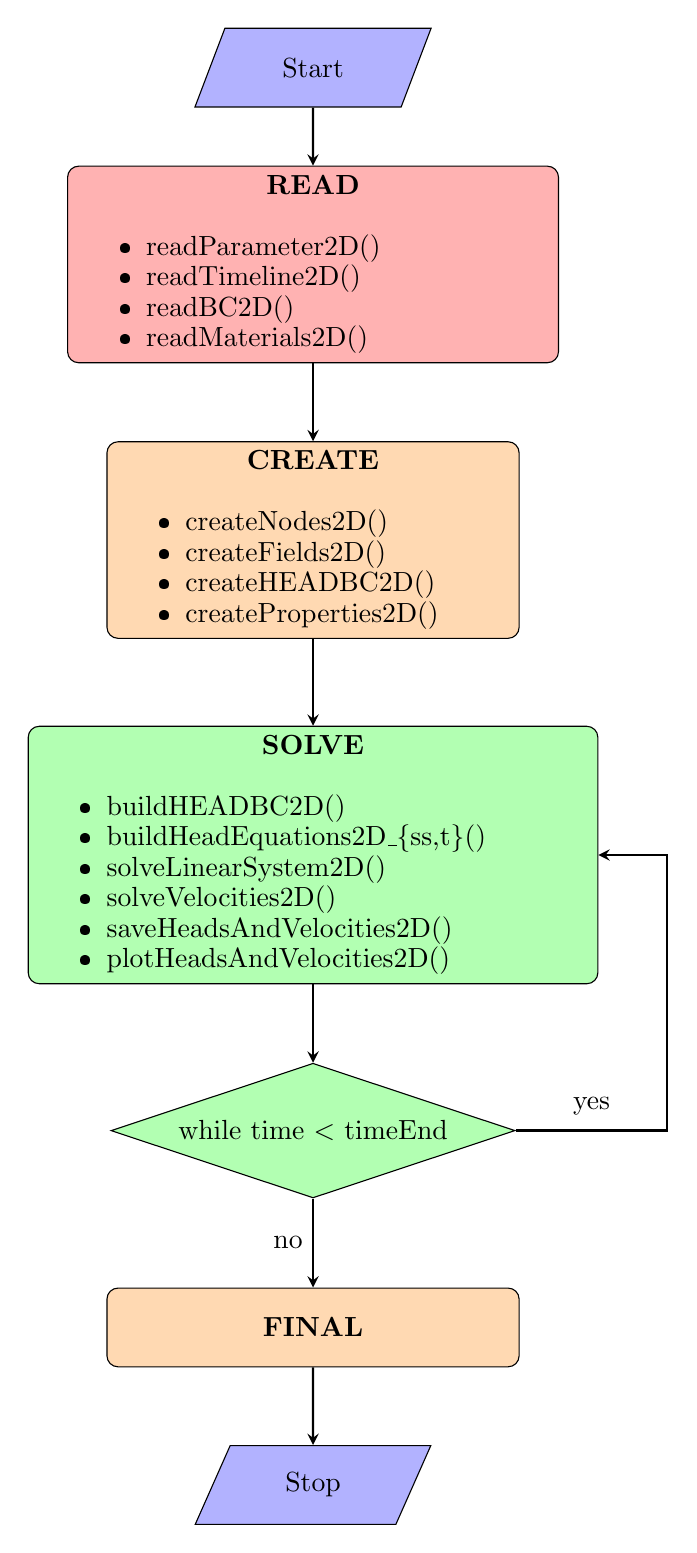
\begin{tikzpicture}[node distance=2cm]

\node (start) [startstop] {Start};

\node (read) [io, below of=start, yshift=-0.5cm] {{\bf READ} \\
\begin{itemize}
\setlength\itemsep{-0.5em}
\item readParameter2D()
\item readTimeline2D()
\item readBC2D()
\item readMaterials2D()
\end{itemize}
};
\draw [arrow] (start) -- (read);

\node(create)[create, below of=read, yshift=-1.5cm]{{\bf CREATE} \\
\begin{itemize}
\setlength\itemsep{-0.5em}
\item createNodes2D()
\item createFields2D()
\item createHEADBC2D()
\item createProperties2D()
\end{itemize}
};
\draw [arrow] (read) -- (create);

\node(run)[run, below of=create, yshift=-2cm]{{\bf SOLVE} \\
\begin{itemize}
\setlength\itemsep{-0.5em}
\item buildHEADBC2D()
\item buildHeadEquations2D\_\{ss,t\}()
\item solveLinearSystem2D()
\item solveVelocities2D()
\item saveHeadsAndVelocities2D()
\item plotHeadsAndVelocities2D()
\end{itemize}
};
\draw [arrow] (create) -- (run);

\node (timeloop) [decision, aspect=3, below of=run, yshift=-1.5cm] {while time $<$ timeEnd};
\draw [arrow] (run) -- (timeloop);

\draw [arrow] (timeloop) --  node[anchor=east, above=2pt ] {yes} ++(4.5,0) |- (run);

\node(final)[create, below of=timeloop, yshift=-0.5cm]{{\bf FINAL} };
\draw [arrow] (timeloop) -- node[anchor=east] {no} (final);

\node (stop) [startstop, below of=final, yshift=-0.0cm] {Stop};
\draw [arrow] (final) -- (stop);

\end{tikzpicture}
\end{document}  
